\documentclass[letterpaper,10pt,titlepage,draftclsnofoot,onecolumn,onesided] {IEEEtran}
\usepackage{listings}
\usepackage{underscore}
\usepackage[bookmarks=true]{hyperref}
\usepackage[utf8]{inputenc}
\usepackage[english]{babel}
\usepackage{titling}
\usepackage{graphicx}
\usepackage[noadjust]{cite}
\nocite{*}
\graphicspath{ {img/} }
\usepackage{abstract}

% C: I added this package for the definitions portion of the document
\usepackage{amsthm}

\newcommand{\namesigdate}[2][4cm]{%
  \begin{tabular}{@{}p{#1}@{}}
    #2 \\[2\normalbaselineskip] \hrule \\[0pt]
    {\small \textit{Signature}} \\[2\normalbaselineskip] \hrule \\[0pt]
    {\small \textit{Date}}
  \end{tabular}
}
\newcommand{\studentnamesigdate}[2][4cm]{%
  \begin{tabular}{@{}p{#1}@{}}
    #2 \\[2\normalbaselineskip] \hrule \\[0pt]
    {\small \textit{Signature}} \\[2\normalbaselineskip] \hrule \\[0pt]
    {\small \textit{Signature}} \\[2\normalbaselineskip] \hrule \\[0pt]
    {\small \textit{Signature}} \\[2\normalbaselineskip] \hrule \\[0pt]
    {\small \textit{Signature}} \\[2\normalbaselineskip] \hrule \\[0pt]
    {\small \textit{Date}}
  \end{tabular}
}

\hypersetup{
    bookmarks=false,    % show bookmarks bar?
    pdftitle={Design Document},    % title
    pdfauthor={Cramer Smith, Sam Lichlyter, Eric Winkler, Zach Schneider},                     % author
    pdfsubject={Design Document},                        % subject of the document
    pdfkeywords={IFT, Design, Postal}, % list of keywords
    colorlinks=true,       % false: boxed links; true: colored links
    linkcolor=black,       % color of internal links
    citecolor=black,       % color of links to bibliography
    filecolor=black,        % color of file links
    urlcolor=blue,        % color of external links
    linktoc=page            % only page is linked
} 

% Document Title:
\def\doctitle{A Tool to Automatically Organize the Structure of a Codebase Using Information Foraging Theory Design Patterns}
\def\doctype{Design Document}
\def\team{Team Postal | Group \#38}

\markboth{Oregon State University}{\doctitle}

\begin{document}

\title{\Huge{\bfseries{\textsf{\doctitle}}}\\\textsf{\Large{\doctype}}\\\textsf{\large{\team}}}
\author{Cramer Smith, Sam Lichlyter, Eric Winkler, Zach Schneider}

\maketitle
\vfill
%\begin{abstract}
%\end{abstract}
\vfill

\pagebreak

\tableofcontents

\pagebreak

A note for grading: Each major component and their subcomponents was covered by a different member of the team in this document. 
\begin{itemize}
\item IDE/Extension -- Cramer Smith
\item Parser -- Sam Lichlyter
\item UI -- Eric Winkler
\item Data Handling -- Zach Schneider
\end{itemize}
The majority of the design details on these components takes place in section 5 of this document. The preceding details and introductions were distributed amongst the team.

\pagebreak

% 1
\section{Overview}

% 1.1 
\subsection{Scope}
This document will cover the entirety design of the Postal extension written for the Visual Studio Code integrated development environment. 
The focus of the design will be on the four main parts of the extension, and the use of Information Foraging Theory within the extension.
The four parts of the extension design are the parser, the data structure, the interface with Visual Studio Code and the user interface.
The document with go through each of these parts and describe in detail how each will be implemented and how each part will function.
The Information Foraging Theory Patters that are planned to be explored within the extension are the Specification Matcher, Structural Relatedness, Impact Location, Path Search, and Recollection.
The document will go into more detail as to what these patterns mean and how they will influence the design of the extension.

% 1.2
\subsection{Purpose}
This design document describes the planned design and steps for implementing the Postal extension for Visual Studio Code. 
The team implementing the design will use this document as the blueprint for the implementation of the extension. 

% 1.3
\subsection{Intended Audience}
This document is meant for the design stakeholders. 
The design stake holders include the team implementing the extension, their client, and the teams supervisors. 
The teams supervisors being the people grading the project on the implementation of the designs described within this document.

% 1.4 
\subsection{Conformance}
This document conforms to the IEEE Std 1016-2009.

% 2
\section{Definitions, Acronyms, and Abbreviations}

% 2.1
\subsection{Definitions}
Model-View-Controller\\
A design pattern assigns objects in an application one of three roles: model, view, or controller. 
The pattern defines not only the roles objects play in the application, it defines the way objects communicate with each other. 
Each of the three types of objects is separated from the others by abstract boundaries and communicates with objects of the other types across those boundaries. 
The collection of objects of a certain MVC type in an application is sometimes referred to as a layer for example, model layer.\cite{appleMVC} \\
Integrated Development Environment\\
A software application that provides comprehensive facilities to computer programmers for software development. \\
dictionary \\
An abstract data type composed of a collection of (key, value) pairs, such that each possible key appears at most once in the collection.

% 2.2
\subsection{Acronyms}
VSC \\
Visual Studio Code. Visual Studio Code is the IDE for which the Postal Extension is being built. \\
IDE \\
Integrated Development Environment. \\
UI \\
User Interface. \\
MVC \\
Model-View-Controller


% 3
\section{Conceptual Model for Software Design Descriptions}
This software will be loosely written with a model view control design pattern.
It is loosely MVC because it is an extension and some of the view will be out of the control of the extension, but the main parts of the extension will fill these MVC roles.
The model will be the data structure that will be used to represent the parsed files. 
The IDE and the user interface that the extension creates will be the view and be dependent on each other.
The control will be the event handlers and the IDE, as these parts take and interpret the users actions that affect the data structure and in turn the UI.

% 3.1
\subsection{Software Design in Context}
The extension is designed to help novice web developer with organizing and create cleaner HTML and CSS code. 
To accomplish this, the design of the extension will contain a UI, a number of parsers for different languages, and a data structure to keep track of relevant information from the user's files..
The parsers and the extension's UI will need to communicate between each other and VSC.
The communication between VSC and the parser will go though the data structure as VSC passes text to the parser and the parser populates information within the data structure.

% 4
\section{Design Description Information Content}

% 4.1
\subsection{Introduction}
The following paragraphs will detail all primary pieces of this design document and the design of the Postal Extension. 
Information concerning who is responsible for the various facets of this piece of software, the major components of the software, the viewpoints from which these components will be designed, and the languages with which the components will be described will be detailed in the following sections.

% 4.2
\subsection{SDD Identification}
This document identifies the various components of the Postal VSCode Extension and how they function together. These components exist of the following:
\begin{itemize}
\item IDE
\item Parser
\item UI
\item Data Handling
\end{itemize}

% 4.3
\subsection{Design Stakeholders and Their Concerns}
The design stakeholder for this design are the development team, the client, and the supervisors.
The development team will be using this as a blueprint for the implementation of the postal extension. 
The client will use this to check that the development team is headed in the right direction as to what the client is hoping for a final product.
The supervisors will use this document to grade how we implement and design the project.

% 4.5
\subsection{Design viewpoints}
This document has organized into five design viewpoints that will be used to describe the Postal Extension.
These viewpoints are as follows:
\begin {itemize}
\item Composition Viewpoint
\item Logical Viewpoint
\item Interaction Viewpoint
\item Information Viewpoint
\item Interface Viewpoint
\end {itemize}

% 4.6
\subsection{Design Elements}
The chief design elements present in the Postal extension can be summed into the following categories: the IDE/extension functions, the UI entities and functions, the Parser and data handling.
Many of the attributes of the IDE and extension are related to functionality provided by VSC or functionality that this extension will provide. 
The UI is broken down into the File Map and Error List viewer, which provide the user with relevant information on their project.
The Parser acquires data from the user's files and transfers that information to the data handler functions.
The data handler entities and functions provide the UI with up to date information for the user to view.
These design elements will be described within the context of specific design viewpoints.

% 4.8
\subsection{Design Rationale}
The Postal Extension project will attempt a pseudo agile design style focusing on incremental releases and feature implementation.
As this project has a very short time line, it is important to release and mature key features before lower priority features. 
It an attempt to avoid over-engineering and feature creep, the project has set relatively simple minimal goals that must all be completed before the project can move on to more complex ones.
We hope that by setting this restriction, we can guarantee at minimal feature release and meet our time line goals.
The current minimal features are (as of 12/01/2016) already under implementation and are expected to be completed before January of 2017.


% 4.9
\subsection{Design Languages}
The following document makes us of Entity-Relationship (ER) diagrams to represent information and data structures and UML diagrams for displaying system components. 

% 5.1
\section{Introduction of Design Viewpoints}
The design components of the Postal Extension will each be addressed and detailed by at least one of the following design viewpoints: Composition Viewpoint, Logical Viewpoint, Interaction Viewpoint, Information Viewpoint and Interface Viewpoint.
In each of the following sections, each viewpoint will be briefly described, the design concerns of that viewpoint introduced, then the design elements discussed.

\section{Composition Viewpoint}
The Composition viewpoint describes the way the design subject is (recursively) structured into constituent
parts and establishes the roles of those parts. 
\subsection{Design Concerns}
Show the major components of the extension and their general, high-level functions.
\subsection{Design Elements}
	\begin{figure}
                 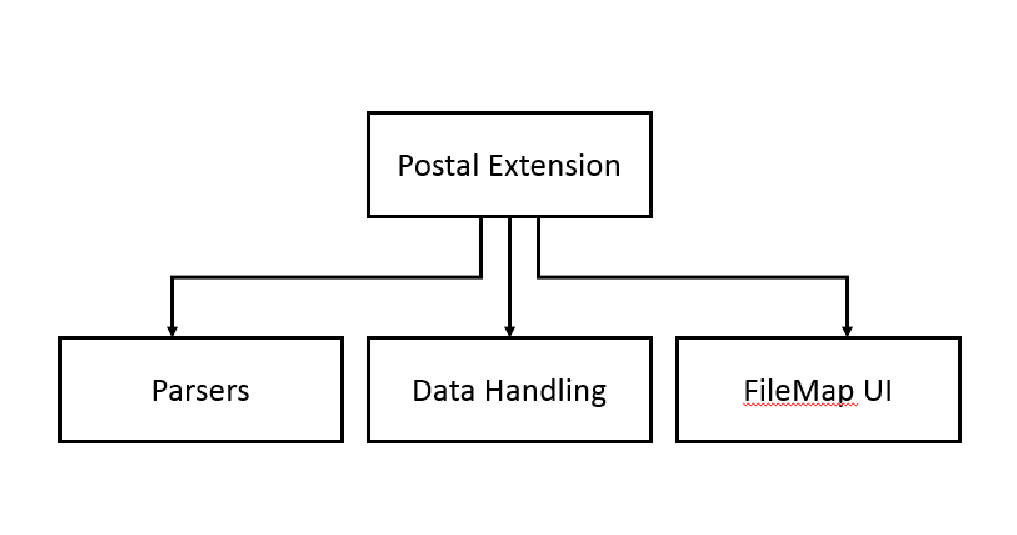
\includegraphics[width=300px]{CompositionUMLEPS.eps}
                 \caption{Components of the Postal Extension}
      		\end{figure}
	\subsubsection{Extension}
	Type: system
	Description: The design of the extension is meant to help new web developers make better design decisions when writing HTML and CSS code.
	The extension is to be built on top of the Visual Studio Code IDE and the extension will be the completion of the all the parts that are described within this document. 
	The parts of the extension are as follows:
	\begin{itemize}
	\item Visual Studio Code and how it interacts with the extension.
	\item The parsers that take the language and parse the languages and find errors.
	\item The data structure that is used to store the information that the parser finds.
	\item The UI that the extension adds to the users. 
	\end{itemize}
	All of these components make up the entirety of the extension, and they will be described more entirely within this document. 
	
	\subsubsection{Parser}
	Type: component
	Description: 
	The parser is the primary logic of the Postal extension. 
	It is responsible for gathering and analyzing all the data from the user and generating the data that will go into the data structure.
	It will parse through each file and check if the user's code violates any best practices of HTML, CSS, JavaScript, or PHP. 
	It will also generate the file map by looking at what HTML pages are linked to other HTML pages.
	The parser will update the data structure with only the data that was changed most recently.
	For example if a user saves a file, only that file be parsed again and its new data sent to the data structure.
	Similarly if a user saves multiple files at the same time then only those file would be parsed and sent to the data structure.
	
		
	
	\subsubsection{File Map and Error List UI}
	Type: component
	\\
	Description: The FileMap and Error List UI is the only GUI included in the Postal Extension. 
	The GUI has two primary responsibilities: 
	\begin{itemize}
	\item Displaying a visualization of the user's project directory in the form of a graph of interconnected nodes.
	\item Displaying a list of the Broken Rules in the project directory detected by the extension parser.
	\end{itemize}
	Both subcomponents of the GUI will offer a degree of interactivity with the user. 
	The GUI will be launched from the Visual Studio Code IDE through the use of the VS Code Command Line.
	When Launched, the UI Component will interface with the data handling component to retrieve the information necessary to construct the file map and error list.

	
	\subsubsection{Data Handling} 
	Type: component
	Description: The information source from which the UI derives its data will be called the data structure. 
	The data structure is a dictionary of file nodes and links collected by the Parser for the project currently loaded into VSC. 
	The file nodes within the data structure will contain information related to all the files in the projects, as well as error data detected by the parser.
	The data structure will be serialized into structured JSON objects by the JSON.stringify function and saved to a file. \cite{stringify}
	This JSON file will be the direct source from which the UI obtains its data.

	
	
% 5.4
\section{Logical Viewpoint}
The purpose of the Logical viewpoint is to elaborate existing and designed types and their implementations
as classes and interfaces with their structural static relationships. This viewpoint also uses examples of
instances of types in outlining design ideas. 
\subsection{Design Concerns}
Show the abstractions at the class and datatype level that are required for each component. 
\subsection{Design Elements}


	\subsubsection{Parser}
	The Parser will be implemented using Perl and the HTMLTokeParserSimple library\cite{htmltokeparser}.
	This library tokenizes HTML files into their basic parts such as the tags in it as well as the various attributes within each tag.
	The parser will use this information to grab links from the pages and determine which pages are linked to each other.
	It will also look at a higher level of the users code structure and determine if they are violating any best practice thus creating Broken Rules. 
	
	The Broken Rules will be determined by going through the W3C best practices list and determining what types of things should exist in each file type. 
	For example having only the structure of the website in the HTML pages and having all the styling in the CSS pages. 
	We will then format rules in which our parser will interpret and return error messages to the user if they broke a best practice thus generating a Broken Rule.\cite{w3c}
	

	\subsubsection{File Map and Error List UI}
	The User Interface system will consist of two main components: The File Map and the Error List. 
	Both of these components will be bundled together into a single screen. 
	This screen will implemented in an electron application window. 
	Electron is a platform used to create desktop applications as if they were websites. \cite{Electron}
	The user interface will then be implemented using JavaScript, HTML and CSS.
	
	\subsubsection{FileMap}
	Type: Interface
	Description: 
	The file map will be a graphic representation of the of the user's project solution. 
	It will appear as a heirarchical graph of interconnected nodes where the nodes represent a file or directory in the user's project directory and an edge represents some link (defined in the parser section) between the two files.
	The location of the nodes in the heirarchy will reflect its postion in the project's directory.
	This web will feature nodes of different sizes and will allow the user to zoom and pan the view.
	The file map will be generated from the above mentioned data structure. 
	On execution of a Visual Studio Code command, the Electron application will fetch the data structure and generate the file map by traversing the 'FileStruct' graph structure.
	When a Node is generated it will have several visual attributes which will be acquired from the data structure:
	\begin{itemize}
	\item The size of the node will be based on the number of links to that object (size of the links[] array). 
	\item A color corresponding to the type of file. Color values will be based on the VSC color scheme for aesthetic reasons. 
	See below table.
	\end{itemize}
	\begin{tabular}{| c | c |}
	\hline
	Color & File Type\\
	\hline
	Blue & HTML\\
	Purple & CSS\\
	Green & JavaScript\\
	Yellow & Image\\
	Light Blue & PHP\\
	Grey & Undefined\\
	\hline
	\end{tabular}
	\\
	
	The name of the node will be retrieved from the file struct name field and will be displayed as text inside of the node.
	An red circle will appear on the node if there are errors within the FileStruct for that node. In other words, if the size of the errors[] array within the FileStruct is not zero.
	The file map will be rendered within its own div using the vis.js library 'Network' module. 
	The Library by default includes the rendering, panning and zooming functionality. \cite{visjs}
	
	\subsubsection{Error List}
	Type: Interface
	Description: 
	The error list will display all errors currently in the project directory in the form of a vertical list. 
	These errors will be retrieved when the UI opens from the same data structure is being generated. 
	These errors will be retrieved in a per node fashion and will also be grouped in the error list in the same order. 
	\\
	The error list will exist to the side of the file map in the same electron application screen. 
	The list will allow the user to scroll when the number of errors result in the list exceeding the electron window height. 
	When an error in the list is hovered over, these errors will highlight the corresponding node in the file map by changing the color value of said node. 
	When an error in the list is clicked, the extension will open the file in Visual Studio Code's text editor and scroll to line where the error exists.
	The error list will be in its own div and scrolling functionality will be achieved through the use of JQuery Advanced News Ticker. \cite{newst}
	
	\subsubsection{Data Handling}
	Data handling within the Postal Extension consists of three main entities or processes: the data structure, serialization of the data structure and the storage of the data structure in a JSON file.
	The data structure is a dictionary of file nodes, stored as JavaScript objects. These JavaScript objects come from the Parser parsing the currently loaded project for links and errors.
	The data structure can be considered the live version of the project data, as its dictionary is updated by the parser every time the project is saved. 
	Once the data structure is updated, its data will be compared with the now out-of-date JSON file to identify which file nodes were changed.
	The comparison of JSON and JavaScript object will be done with the Lodash library's deep object compare function.
	The information concerning which nodes were changed will be passed to the UI elements, once it has been serialized to the file.
	The nodes changed in the data structure will then be serialized into JSON using the JSON.stringify function built into JavaScript.
	This JSON will be saved to a file, which can further be read by the UI functions for updating. \cite{stringify} \cite{lodash}
	
% 5.10
\section{Interaction Viewpoints}
The interaction viewpoint defines strategies for interaction among entities, regarding why, where, how, and
at what level actions occur. Most of these interactions are between predefined events and event listeners.
\subsection{Design Concerns}
The primary design concerns from an interaction viewpoint in the Postal Extension are within the IDE and its interactions with the rest of the components of the software.
Additionally, within the data handling elements of this extension, how the data passes from the data structure to JSON files is also an important interaction.

\subsection{Design Elements}

\subsubsection{IDE}	
	There are three main interactions that happens on the specific IDE events; the parsing of the files ,the opening of the custom extension UI, and the opening of an error object.
	The first of these events is the parsing of files. 
	There are several actions that occur within VSCode that will initiate the extension parsing and interpreting process.
	These specific events that will have specific event listeners. 
	Each event will trigger a specific type of the same parsing process.
	These events are when the user starts the extension, when the user explicitly saves one or all the files, and when the user closes the application.
	When the user starts Postal the extension will first initial parsing and create the data structures that will serve as a reference for the next continuation of the extension processing.
	The first parsing will be set in motion by the built-in activate function with the extension initialization. 
	After the initialization whenever the user saves the files the extension is going to parse the files and get the necessary information from the new parse. 
	This will continue after every manual save.
	The extension will only continue on the explicit manual saves, meaning only when the user to saves the files, rather then when VSC auto saves. 
	Once the user saves the files the inPerSaveDocument listener will be acted upon.\cite{VSCodeDocumentation}
	This specific event will allow the extension parser to read the files contents before the file is actually saved.
	This will allow for the extension to possibly format the user's code before it is saved.
	The third even is when the user closes the VSC application or kills the extension then the deactivate listener will do one last parse of the files so that the user will be where they left next time they 	comeback to the project.
	These three events should be able cover the major of instances when the extension is expected to be iterated.
	
	The extensions custom UI will open on the user invoked 'Postal' Command. 
	This command can be run from the VSC command pallet and will read the most recent parse of the datastructure. 

	An error object is the location of what the extension finds and identifies as an error.
	These error will consist of improper HTML and CSS practices. 
	These errors will be listed in the custom UI, and if the user interacts with the error object the extension should navigate the user to the location of the error.
	The extension will do this with openTextDocument, to first open the document that has the error. 
	Once the extension opens the file it can then get the specific words that are part of the error and change the background color using the background color property. \cite{VSCodeDocumentation}
	This will hopefully give the user a good idea of where the user has created the error and the errors information text will give the user an idea of what mistake they made and how it can be fixed.

\subsubsection{Data Handling}
	Most major actions within the data handling entities and functions are reliant on the Parser being called and providing updated data.
	The data structure is updated when files are saved and reparsed. 
	Information on which file nodes within the data structure dictionary were changed is also identified when a reparse occurs.
	The likewise is true with serialization of the data structure to the JSON.
	Each Parser call results in each data handling function taking place. 
	Other components that rely on information within the data handling scope are then also reliant on the Parser for updates.
	

	
\section{Information Viewpoint}
The Information viewpoint is applicable when there is a substantial persistent data content expected with
the design subject. 
\subsection{Design Concerns}
The primary element of concern from an Information Viewport in the Postal Extension is the data structure data layout. 
The main objects contained in the data structure are detailed below.
\subsection{Design Elements}

	\subsubsection{Dictionary}
	The overall format of the data structure is as a dictionary, that is, a collection of key-value pairs. 
	The keys will be identifiers and the values will be specific file nodes. 
	At this point in time, the exact implementation of the dictionary keys has not been determined, but it will likely be some sort of hash table.
	The values, the file nodes, will contain the relationship and error data for all files in the loaded project.
	\subsubsection{File Nodes}
		A file node will be representative of an individual file in the loaded project. 
		Each file node will contain the name of the file it represents, as well as a numerical identifier for lookups.
		File nodes will be linked to each other according when one file in the project references another. 
		Many files may be linked to many other files.
		The files supported by default will be HTML, CSS JavaScript, PHP and image files.
		
	\subsubsection{Errors}
		File nodes will also contain any and all errors present in their respective files.
		These errors will have a unique identifier, the error message or type of error occurring, and the line number the error occurs on.
		File nodes may have multiple errors, but each error is only linked to one file node.

	\begin{figure}
        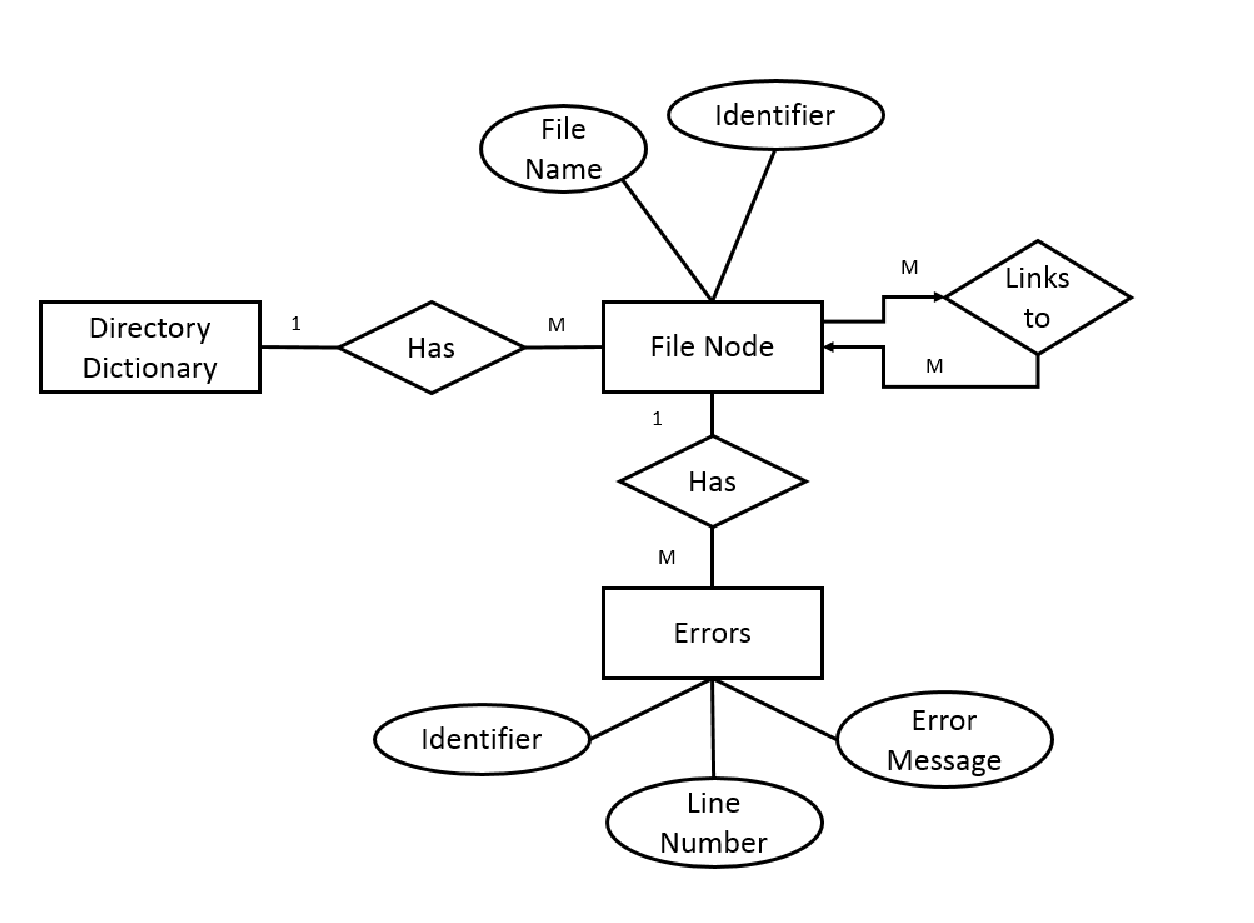
\includegraphics[width=300px]{InformationERDEPS.eps}
        \caption{A visual representation of the data structure.}
    \end{figure}
		
		
		
\section{Interface Viewpoints}
The Interface viewpoint provides information designers, programmers, and testers the means to know how
to correctly use the services provided by a design subject. This description includes the details of external
and internal interfaces not provided in the SRS. This viewpoint consists of a set of interface specifications
for each entity. 
\subsection{Design Concerns}
Identifies the interfaces that the components of the framework expose or require to achieve their
functionality. 
\subsection{Design Elements}

		\begin{figure}
                 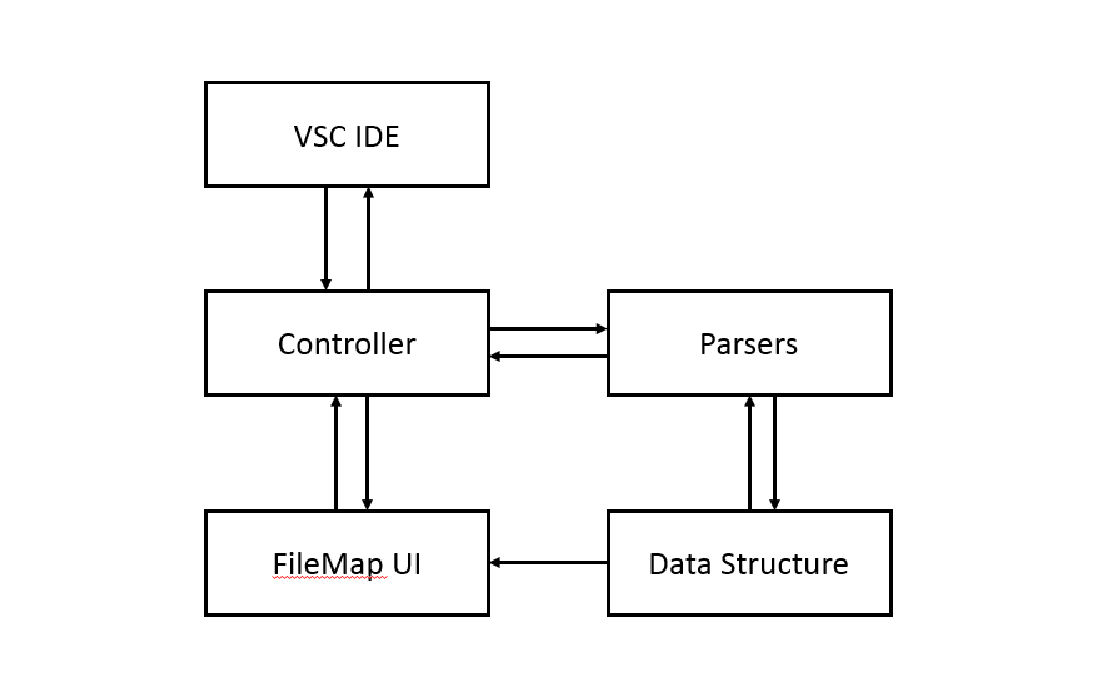
\includegraphics[width=300px]{InterfaceUMLEPS.eps}
                 \caption{Exposed interfaces}
      		\end{figure}

	\subsection{IDE}
		\subsubsection{Exposes}
			\begin{itemize}
			\item Opening the GUI give the user an interface in which they can interact and see the information that they are looking for from the Postal extension.
			\item That information includes the file structure and how they relate to each other, as well as the possible errors. 
			\end{itemize}
		\subsubsection{Requires}
			\begin{itemize}
			\item The parsing of the file is the process that populates the information that is displayed in the UI.
			\item The operations are signaled to start on certain event listeners.
			\end{itemize}
			
	\subsection{Parser}
		\subsubsection{Exposes}
			\begin{itemize}
			\item Parsing for links and Broken Rules
			\end{itemize}
		\subsubsection{Requires}
			\begin{itemize}
			\item The parser will be triggered when the user saves files, and only those files will be parsed. 
			It will also parse on first launch of the extension.
			\item Get Data from the Data Structure
			\end{itemize}
	
	\subsection{Data Structure}
		\subsubsection{Exposes}
		\begin{itemize}
			\item Get Data
			\\
			The data structure has its dictionary of file nodes updated when the Parser reparses the loaded project. 
			The data structure gets its data from the parser when Get Data is called.
		\end{itemize}
		\subsubsection{Requires}
		\begin{itemize}
			\item Load Data (Files)
			\\
			The data structure will compare its updated data with the data stored in the JSON file. 
			In order for this to occur, the data structure must make use of JSON.parse and the deep object compare as part of the Load Data function. \cite{stringify}
			\item Parse (Parsers)
			\\
			The data structure will only have its data updated when the Parse function is called.
			\end{itemize}
	\subsection{User Interface}
		\subsubsection{Exposes}
		\begin{itemize}
			\item Error Navigation 
			When the user clicks on an error item in the error list, The UI component will interface with the VS Code IDE API in order to navigate the user's screen to the file and line number of the error.
			\item User-FileMap Interaction
			The User has several options to interface with the File Map. 
			When the user scrolls a mouse wheel, the file map will zoom and expand the size of the file nodes.
			If the user clicks and drags on the white space in the background of the file map, the GUI view will pan and render/discard file nodes that are off screen.
			If the user clicks on a file node and drags, the UI will simulate two dimensional physics and will warp the file map in response to the users movements.
			The three above features can all be achieved through the use of the vis.js API.
		\end{itemize}
		
		\begin{figure}
                 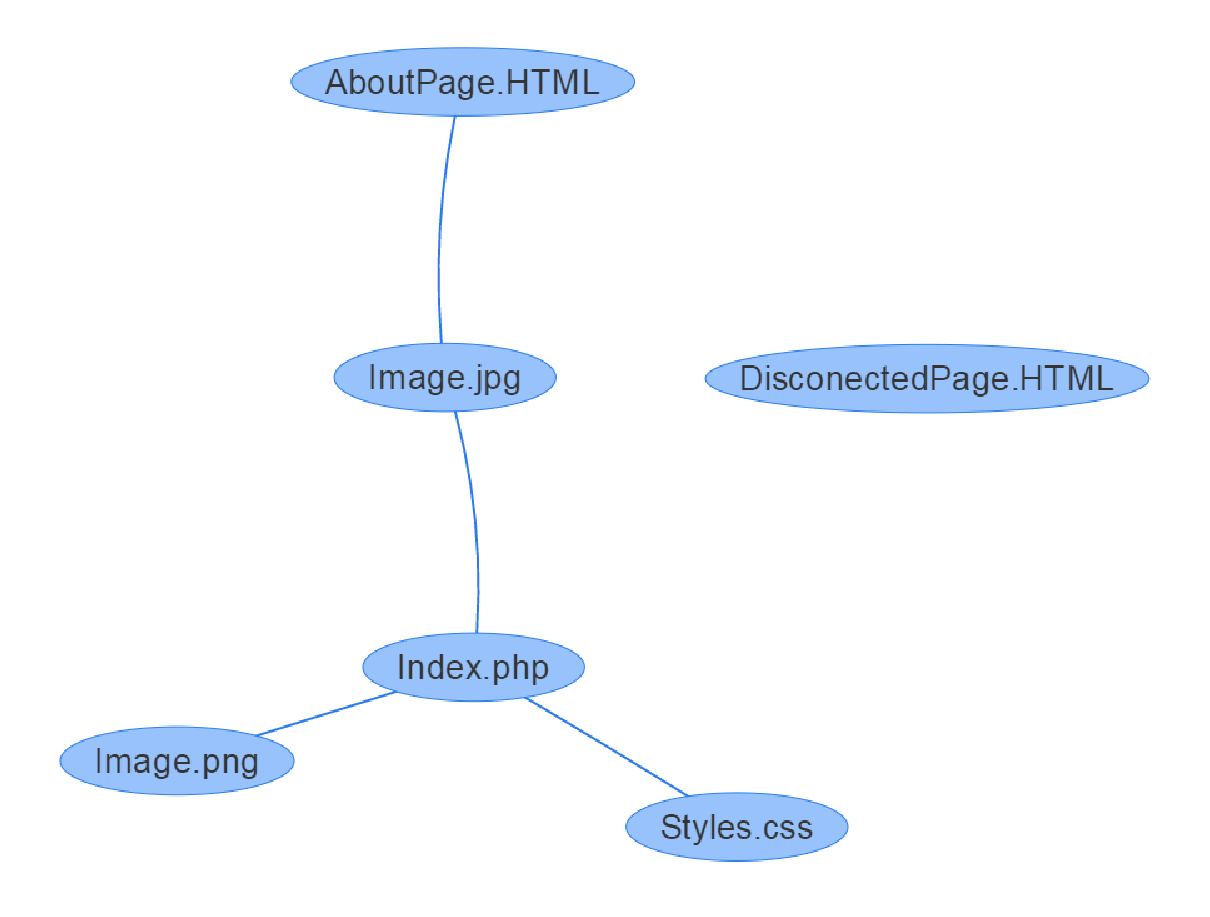
\includegraphics[width=300px]{UIMockupEPS.eps}
                 \caption{Mockup of the user interface}
      		\end{figure}
		
		\subsubsection{Requires}
		\begin{itemize}
			\item Get Data (data structure)
			\item The UI will need to use the command that is used by the user to view the file map and the GUI.
		\end{itemize}
		
	\subsection{Files}
		\subsubsection{Exposes}
		\begin{itemize}
			\item Load Data
			The JSON.parse function will be utilized to pull data from the JSON file. 
			Once the information about the file nodes from the data structure are pulled from the JSON file, it will be compared to the current data structure values to identify which links or errors have changed. \cite{stringify}
			\item Save Data
			Once parsed data from the Parser is transferred to the data structure using the Get Data functionality, this data will be serialized into a JSON file with the JSON.stringify function built into JavaScript.
		\end{itemize}
		\subsubsection{Requires}
		\begin{itemize}
			\item Get Data (data structure)
			It is necessary for the data structure to obtain data from the Parser each time it parses so that this data can, in turn, be saved to the JSON file.
		\end{itemize}


% Annex A  Bibliography
% Annex B  Conforming design language description
% Annex C  Annex C Templates for an SDD

%\section{Conclusion}


\pagebreak
\bibliographystyle{IEEEtran}
\bibliography{design}
\pagebreak

\namesigdate{Client Signature} \hfill 
\studentnamesigdate[4cm]{Student Signatures}
\end{document}
